%----------------------- Introduction ----------------------------
\chapter{Introduction}
\label{ch:1}


By mid-1968 the term Software Engineering was coined at NASA by Margaret Hamilton \cite{first_sw_engineer}. During that time more than 400 people were working on Apollo’s software, because software was how the US was going to win the race to the moon. As it turned out, of course, software was going to help the world do so much more \cite{mcmillan_her_nodate}. 

At that time, programming meant punching holes in stacks of punch cards, which would be processed overnight in batches on a giant computer that simulated the Apollo lander’s work. Everything needed to be tested precisely \cite{mcmillan_her_nodate}.

One day, Margaret’s daughter was playing with the command module simulator’s display-and-keyboard unit and as she toyed with the keyboard, an error message popped up. Lauren had crashed the simulator by somehow launching a pre-launch program called P01 while the simulator was in mid-flight. There was no reason an astronaut would ever do this, but nonetheless, Hamilton wanted to add code to prevent the crash.

NASA denied this idea by stating that the astronauts were trained to be perfect and they would not make any mistakes. So Hamilton added certain procedures to the documentation stating what astronauts should and should not do. However, they did mistakes. In the late 1968, an astronaut inadvertently selected a functionality that had wiped out all the navigation data and without that data, the Apollo computer would not be able to figure out how to get the astronauts home. Fortunately, Houston uploaded new navigational data and the Apollo astronauts came home \cite{first_sw_engineer} \cite{mcmillan_her_nodate}.\\

% ----- NASA ends ----- %
\\Testing activities are within the most important tasks of any business, from the world of software to the toothpaste we use, which should be meticulously tested to guarantee quality before being placed in the hands of the user. The objective of this phase is to guarantee quality standards to avoid failures in the product that might lead to catastrophic losses. \textcolor{red}{One of the reasons why this market keeps growing is due to the high costs involved in correcting these failures in advanced stages, however, detecting them in early stages is very profitable \cite{hernandez_history_2020}.
\\ //TODO: Refrasear este paragrafo. Dizer que existe mercado em torno de bugfixing e que detectar os problemas o mais cedo possivel após estes serem introduzidos é o ideal. e depois ver se há alguma coisa na frase que possa ser mantida e que faça sentido.}


% ----- testing ends ----- %

\textcolor{red}{Software requirements play an essential role when designing a system. Requirements are descriptions of how a software product should perform and therefore, should include not only user needs but also those arising from general organizational, government and industry standards \cite{aurum_engineering_2005}.}

The objective of this project is to create a compiler capable of understanding Functional Requirements and automatically generate their test cases. 

\textcolor{red}{
In order to use this application, such software requirements shall be written on a controlled natural language (CNL) that define the functionalities of a software system. This compiler aims to automatically generate high-level tests by parsing and interpreting requirement contents into a Parse tree. Unit tests are not in the scope of the current project. \\
//todo: Isto pode muito bem ser uma intro de uma próxima secção.
}

%----------------------- Problem and Motivation ----------------------------
\section{Problem and Motivation}
\label{sec:problem_and_motivation}

Common requirements engineering activities involve elicitation, interpretation and
structuring (analysis and documentation), negotiation, verification and validation,
change management and requirements tracing. There are several process models
available to describe the requirements engineering process. The process itself is
often depicted in different forms, including linear, incremental, non-linear and spiral models \cite{aurum_engineering_2005}.
Despite the effort to produce requirements, requirement testing can also be a costly and challenging activity. IV\&V teams are independent of the development organization on a technical, managerial, financial, and contractual basis, but have well-established, working relationships with the development organization \cite{noauthor_independent_2013}. Verification and Validation teams are required to gather solid knowledge about software systems and learning technical features and operational concepts on complex systems such as Trains, Satellites or in the area of Avionics can take several time to master. A misunderstood requirement or lack of technical domain can result in tests that fail or in countless hours of back-and-forth communication.
To address this problem, it was thought of a system to store common technical knowledge and capable of automatically generate test specifications given any software requirement as an input.


%----------------------- Objectives ----------------------------
\section{Objectives}
\label{sec:objectives}
It is known that good textual requirements are critical for the creation of successful systems, and heavy and vague natural language is highly discouraged \cite{incose}.
One of the roles of this software program is to guarantee that the requirements of the system under testing are following a predefined grammar [See Section 3] by checking their syntax and whether they are parseable, otherwise, a syntax-error message is generated. On a side note, having the written requirements following a stipulated grammar makes those requirements much easier to understand by the test engineers.
When the requirements are successfully parsed, the conditions and expected results are extracted from them. The required data, to support the test generation process is stored on a knowledge-base in a form of a software signal database.


%----------------------- Schedule ----------------------------
\section{Schedule}
\label{sec:schedule}
This project has been composed by five main activities. Those are illustrated on the following Figure \ref{fig:schedule}.

\begin{figure}[h]
    \centering
    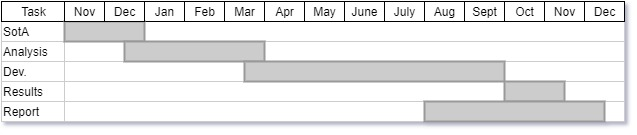
\includegraphics[width=\textwidth]{images/gantt.jpg}
    \caption{Scheduled Activities}
    \label{fig:schedule}
\end{figure}

\begin{itemize}
    \item SotA - State of the art - Study of the existing technologies and scientific advances and how they can contribute to this project.
    \item Analysis - Analysis and problem dismantling - This task consisted of the analysis of the available resources, results from state of the art and \textit{Datasets} e.g. sets of requirements.
    \item Dev. - Development of the solution - Development of the application, capable of understanding requirements, generating test cases, and test artifacts.
    \item Results - Results and further testing - Analysis of the produced results from the developed tool as well as possible adjustments.
    \item Report - Final project Report - Writing a final project report containing the results from all previous phases.
\end{itemize}

\newpage
%----------------------- Starting point ----------------------------
\section{Starting point}
\label{sec:starting_point}

\textit{Sesnando} has kicked-off at Critical Software (CSW) under the management of Dr. João Gabriel Silva. When the current thesis works have started to be carried out, a Railway project was being developed at CSW in increments and in a stable phase, given that it was already operating in passenger service. It has been decided to evaluate the capabilities of \textit{Sesnando} against such project.\\
A new grammar has been designed, specified, accepted and implemented to accomodate the requirements of the target Railway Project. Test Generator and Test Designer have been created under the scope of this thesis and the overall solution evolved to scalable architecture, so that, it can be easily adapted to future projects.
Signal Manager has been developed at CSW by a graduate engineer where several talks have been carried-out about its architecture and design in order to create a consensus with the test generation module.


%----------------------- Scope of this doc ----------------------------
\section{Scope of this document}
\label{sec:document_scope}

The first chapter (Ch. \ref{ch:1}) introduces the current project, its main motivations and objectives in general.\\
The second chapter (Ch. \ref{ch:2}) presents the limitation of this study and how it was conducted.\\
The third chapter (Ch. \ref{ch:3}) presents the state of the art, what are the current scientific advances in this subject, the available tools and technology.
The forth chapter (Ch. \ref{ch:4}) discusses the works done for this project, its requirements and architecture, and it's divided on two main sections, the application life-cycle and the method. The former (Sec. \ref{sec:application_lifecycle}) presents \textit{Sesnando} on a higher level and describes the main functionalities of the software and how to operate it. The latter (Sec. \ref{sec:method}) presents the project in a lower perspective, how its core functionalities have been implemented and the reasons behind it.
The fifth chapter (Ch. \ref{ch:5}) presents the conclusion and the final results from the analysis of this tool in-the-field.
